\FloatBarrier
\noindent The representative gain trajectory must now be examined over a longer horizon to determine what the early increase in semi-major axis actually corresponds to dynamically, and why that favourable behaviour does not persist. The central result is simple to state: the early increase in \(a\) is real, but it is produced mainly by apogee pumping rather than by a clean upward translation of the whole orbit. This increases eccentricity, lowers perigee and concentrates drag loss near perigee; at the same time the inertially fixed sail normal drifts steadily out of alignment with the Sun, so that the SRP forcing which created the gain collapses in magnitude. The second of these effects dominates the late-time behaviour. Together they drive the orbit-averaged energy balance negative at the peak of \(a\), and by day \(75\) the accumulated surplus has been fully erased.

\vspace{5pt}
\par\noindent Figure~\ref{fig:elementsvstime} makes the first part of that breakdown visible directly. For the representative \(800\,\mathrm{km}\) gain case introduced in Section~\ref{sec:existence} (LTAN \(14.0\,\mathrm{h}\), pitch \(+35^\circ\), RAAN \(312.05^\circ\)), the \(75\)-day histories of mean \(a\), apogee altitude, perigee altitude and eccentricity show that the orbit is not lifted uniformly. Apogee grows far more than perigee is preserved, so the early gain develops together with a progressive departure from circularity. The neutral and decay cases are overlaid for comparison: the decay case (LTAN \(0.0\,\mathrm{h}\), pitch \(-30^\circ\)) loses altitude monotonically and re-enters on day \(64.4\), while the neutral case follows an intermediate, drag-like path between the two. Table~\ref{tab:gaincase_longhorizon_summary} collects the corresponding quantities for the gain case.

\begin{table*}[htbp]
\centering
\caption{Long-horizon summary of the representative \(800\,\mathrm{km}\) gain case over the \(75\)-day propagation (\(1069\) orbits). The case corresponds to altitude \(800\,\mathrm{km}\), LTAN \(14.0\,\mathrm{h}\) (RAAN \(312.05^\circ\)), pitch \(+35^\circ\), inclination \(98.31^\circ\), \(e_0=10^{-4}\), sail area \(100\,\mathrm{m^2}\), mass \(m=10\,\mathrm{kg}\), \(C_r=1.7\) and \(C_D=2.2\). Mean (secular) elements are osculating values sampled at ascending-node crossings. All work quantities are specific, i.e. per unit mass (\(m=10\,\mathrm{kg}\)).}
\label{tab:gaincase_longhorizon_summary}
\small
\begin{tabular}{p{4.9cm} p{1.8cm} p{3.2cm} p{1.8cm}}
\toprule
Quantity & Initial & Peak / minimum (day) & Final (day \(75\)) \\
\midrule
Mean semi-major axis, \(a\) [km]
& 7178.168
& 7189.030 (max, day 38.1)
& 7175.479 \\

Peak excursion, \(\Delta a_{\max,75\mathrm{d}}\) [km]
& \multicolumn{3}{l}{\(+10.86\) (day 38.1)} \\

Net change, \(\Delta a_{75\mathrm{d}}\) [km]
& \multicolumn{3}{l}{\(-2.69\)} \\

Apogee altitude [km]
& 801.0
& 912.0 (max, day 43.9)
& 884.7 \\

Perigee altitude [km]
& 799.1
& 708.6 (min, day 48.4)
& 709.9 \\

Eccentricity, \(e\)
& \(1.35\times10^{-4}\)
& \(1.41\times10^{-2}\) (max, day 45.2)
& \(1.22\times10^{-2}\) \\

Cumulative SRP work at day 75 [kJ\,kg\(^{-1}\)]
& \multicolumn{3}{l}{\(+194.5\)} \\

Cumulative drag work at day 75 [kJ\,kg\(^{-1}\)]
& \multicolumn{3}{l}{\(-204.4\)} \\

Cumulative total work at day 75 [kJ\,kg\(^{-1}\)]
& \multicolumn{3}{l}{\(-9.9\)} \\

Work ratio at day 75, \(\left|W_{\mathrm{drag}}\right|/\left|W_{\mathrm{SRP}}\right|\)
& \multicolumn{3}{l}{1.051} \\
\bottomrule
\end{tabular}
\end{table*}

\begin{figure*}[htbp]
    \centering
    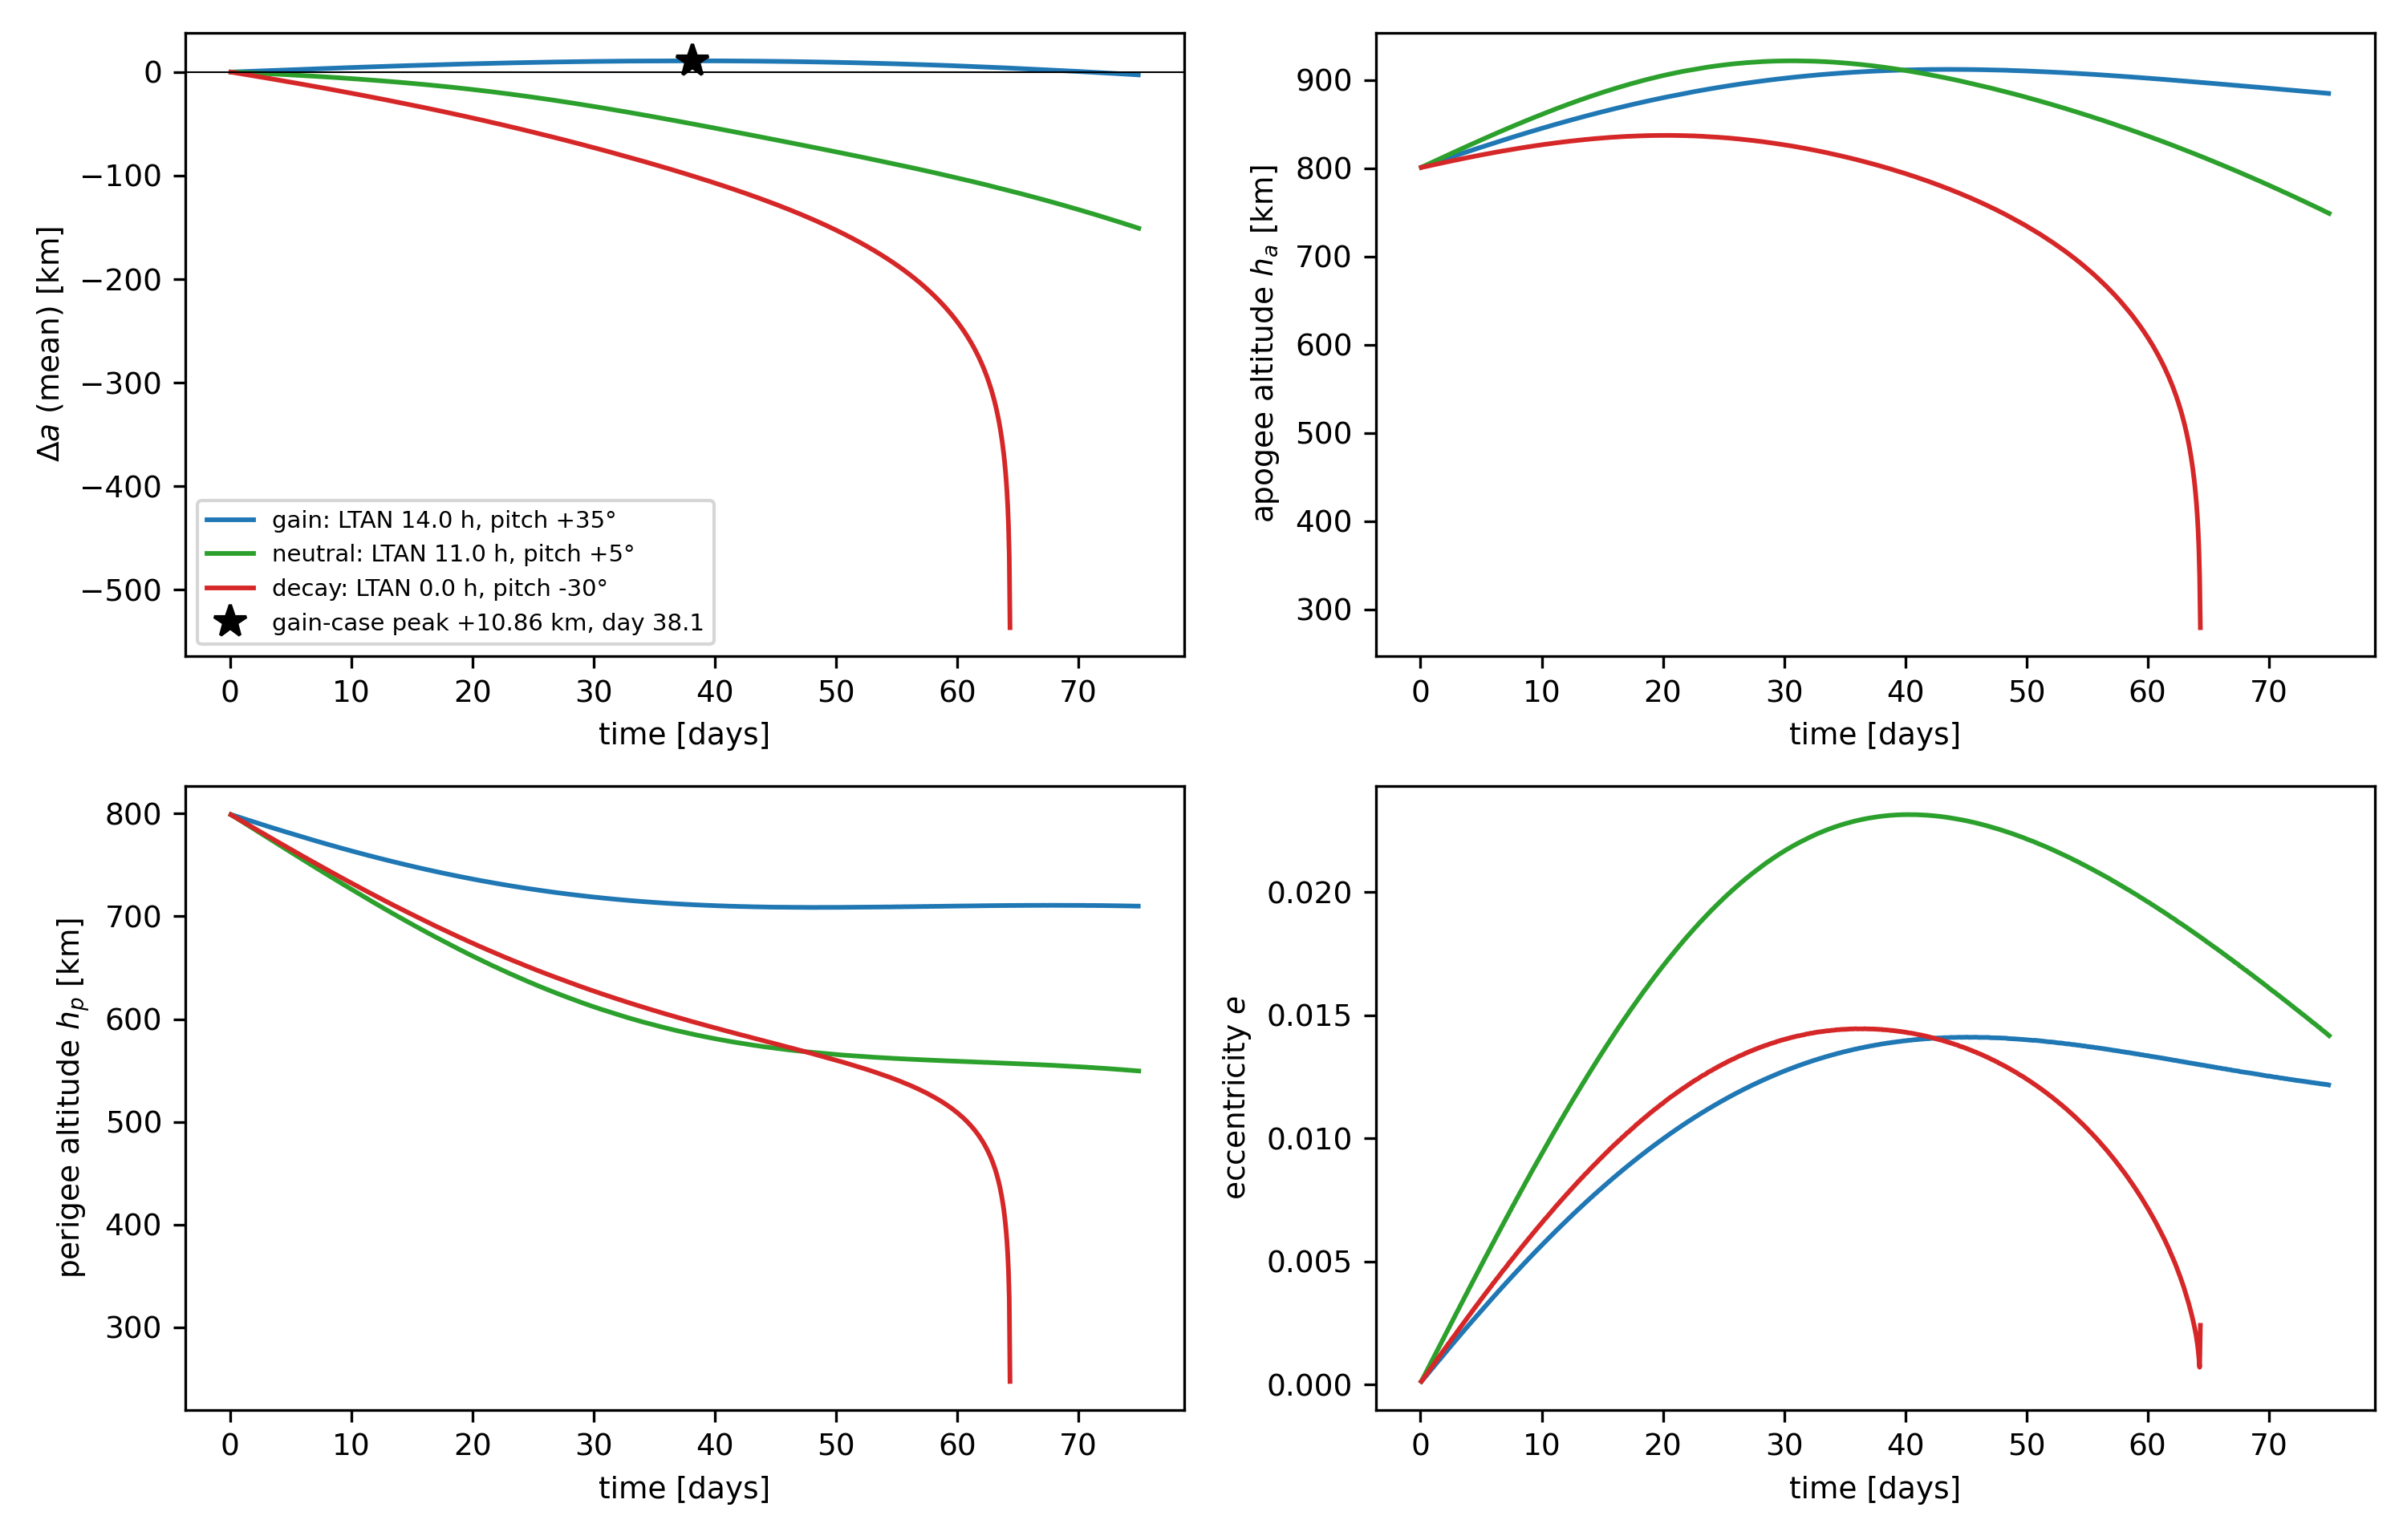
\includegraphics[width=1\linewidth]{Figures/r_elements_75d.png}
    \setlength{\abovecaptionskip}{0pt}
    \caption{Long-horizon evolution of mean orbital elements over \(75\) days for the representative \(800\,\mathrm{km}\) gain, neutral and decay cases: change in mean semi-major axis \(\Delta a\) (with the gain-case peak marked), apogee altitude, perigee altitude and eccentricity. The gain case shows non-monotonic semi-major-axis evolution, strong apogee growth, perigee erosion and eccentricity growth; the decay case re-enters on day \(64.4\).}
    \label{fig:elementsvstime}
\end{figure*}

\vspace{5pt}
\par\noindent The mean semi-major axis of the gain case begins at \(a_0 = 7178.168\,\mathrm{km}\), rises to \(\Delta a(14\,\mathrm{d}) = +5.95\,\mathrm{km}\) at the last ascending node of the \(14\)-day window (day \(13.94\); this is the same trajectory, and the same value, that anchors Section~\ref{sec:existence}), and continues upward more slowly: \(+9.96\,\mathrm{km}\) on day \(28\) and a peak of \(\Delta a_{\max,75\mathrm{d}} = +10.86\,\mathrm{km}\) (\(a = 7189.030\,\mathrm{km}\)) on day \(38.1\). It then declines for the remainder of the propagation, passing \(+10.70\,\mathrm{km}\) on day \(42\), \(+7.59\,\mathrm{km}\) on day \(56\) and \(+0.59\,\mathrm{km}\) on day \(70\), returning to its initial value on day \(71.0\) and finishing at \(\Delta a_{75\mathrm{d}} = -2.69\,\mathrm{km}\) (\(a = 7175.479\,\mathrm{km}\)). The behaviour is therefore explicitly non-monotonic: there is a finite interval of positive excursion lasting roughly ten weeks, but not sustained orbit raising. The short-horizon gain is real, yet by the end of the \(75\)-day window it has been entirely given back.

\vspace{5pt}
\par\noindent The apogee--perigee split shows how that reversal develops. Apogee altitude rises from \(801.0\,\mathrm{km}\) to \(860.4\,\mathrm{km}\) by day \(14\) and \(910.4\,\mathrm{km}\) by day \(38\), peaks at \(912.0\,\mathrm{km}\) on day \(43.9\), and is still \(884.7\,\mathrm{km}\) at day \(75\). Perigee altitude falls from \(799.1\,\mathrm{km}\) to \(751.6\,\mathrm{km}\) by day \(14\) and \(711.3\,\mathrm{km}\) by day \(38\), reaches its minimum of \(708.6\,\mathrm{km}\) on day \(48.4\), and remains depressed at \(709.9\,\mathrm{km}\) at day \(75\). The eccentricity correspondingly grows from \(1.35\times10^{-4}\) to a maximum of \(1.41\times10^{-2}\) on day \(45.2\) and relaxes only slightly to \(1.22\times10^{-2}\). The key point is geometric rather than merely descriptive: the \(+10.86\,\mathrm{km}\) peak in \(a\) is achieved by stretching the orbit, with apogee raised by over \(100\,\mathrm{km}\) while perigee is lowered by about \(90\,\mathrm{km}\), not by lifting it uniformly.

\vspace{5pt}
\par\noindent The physical consequence is that drag loss becomes progressively concentrated near perigee, where the atmosphere is densest. This is the first breakdown pathway visible in the long-horizon outputs: the same evolution that produces the early gain also creates a lower-perigee, more eccentric orbit that is increasingly exposed to atmospheric loss. Eclipse remains essential throughout. Repeating the gain case with the umbra disabled, so that SRP acts around the whole orbit, gives \(\Delta a_{75\mathrm{d}} = -110.5\,\mathrm{km}\), a perigee minimum of \(592.7\,\mathrm{km}\) and \(e_{\max} = 0.0189\): without the eclipse-induced sign selectivity of Section~\ref{sec:existence} the same attitude pumps eccentricity even harder while contributing essentially no net energy, and the orbit ends \(108\,\mathrm{km}\) lower after \(75\) days. The decay case illustrates the same eccentricity pumping with the wrong sign of net work: its eccentricity reaches \(0.0145\) on day \(36.6\), and perigee erosion then runs away to re-entry on day \(64.4\). The former \(700\,\mathrm{km}\) configuration of the original submission (LTAN \(12.266\,\mathrm{h}\), pitch \(24.8^\circ\)) behaves likewise and re-enters on day \(39.5\).

\vspace{5pt}
\par\noindent The cumulative work budget in Figure~\ref{fig:gaincase_cumulative_work_budget} must be read carefully. Over the full \(75\)-day window the cumulative specific SRP work is \(+194.5\,\mathrm{kJ\,kg^{-1}}\) and the cumulative drag work is \(-204.4\,\mathrm{kJ\,kg^{-1}}\), so the cumulative total is \(-9.9\,\mathrm{kJ\,kg^{-1}}\) and \(|W_{\mathrm{drag}}|/|W_{\mathrm{SRP}}| = 1.051\). The total does not fall monotonically: it rises to a maximum of \(+41.3\,\mathrm{kJ\,kg^{-1}}\) on day \(38.1\), the same day on which mean \(a\) peaks, and then declines, crossing zero on day \(71.2\). This is consistent with the semi-major-axis history, since \(\Delta a \simeq (2a^2/\mu)\,W_{\mathrm{total}}\) gives \(-2.6\,\mathrm{km}\) for the day-\(75\) total, matching the node-sampled \(\Delta a_{75\mathrm{d}} = -2.69\,\mathrm{km}\) and the zero crossing of mean \(a\) on day \(71.0\). The regime therefore does more than stop strengthening at late times: the surplus accumulated during the favourable phase is unwound in full, and slightly overshot, within the analysed window.

\begin{figure}[htbp]
    \centering
    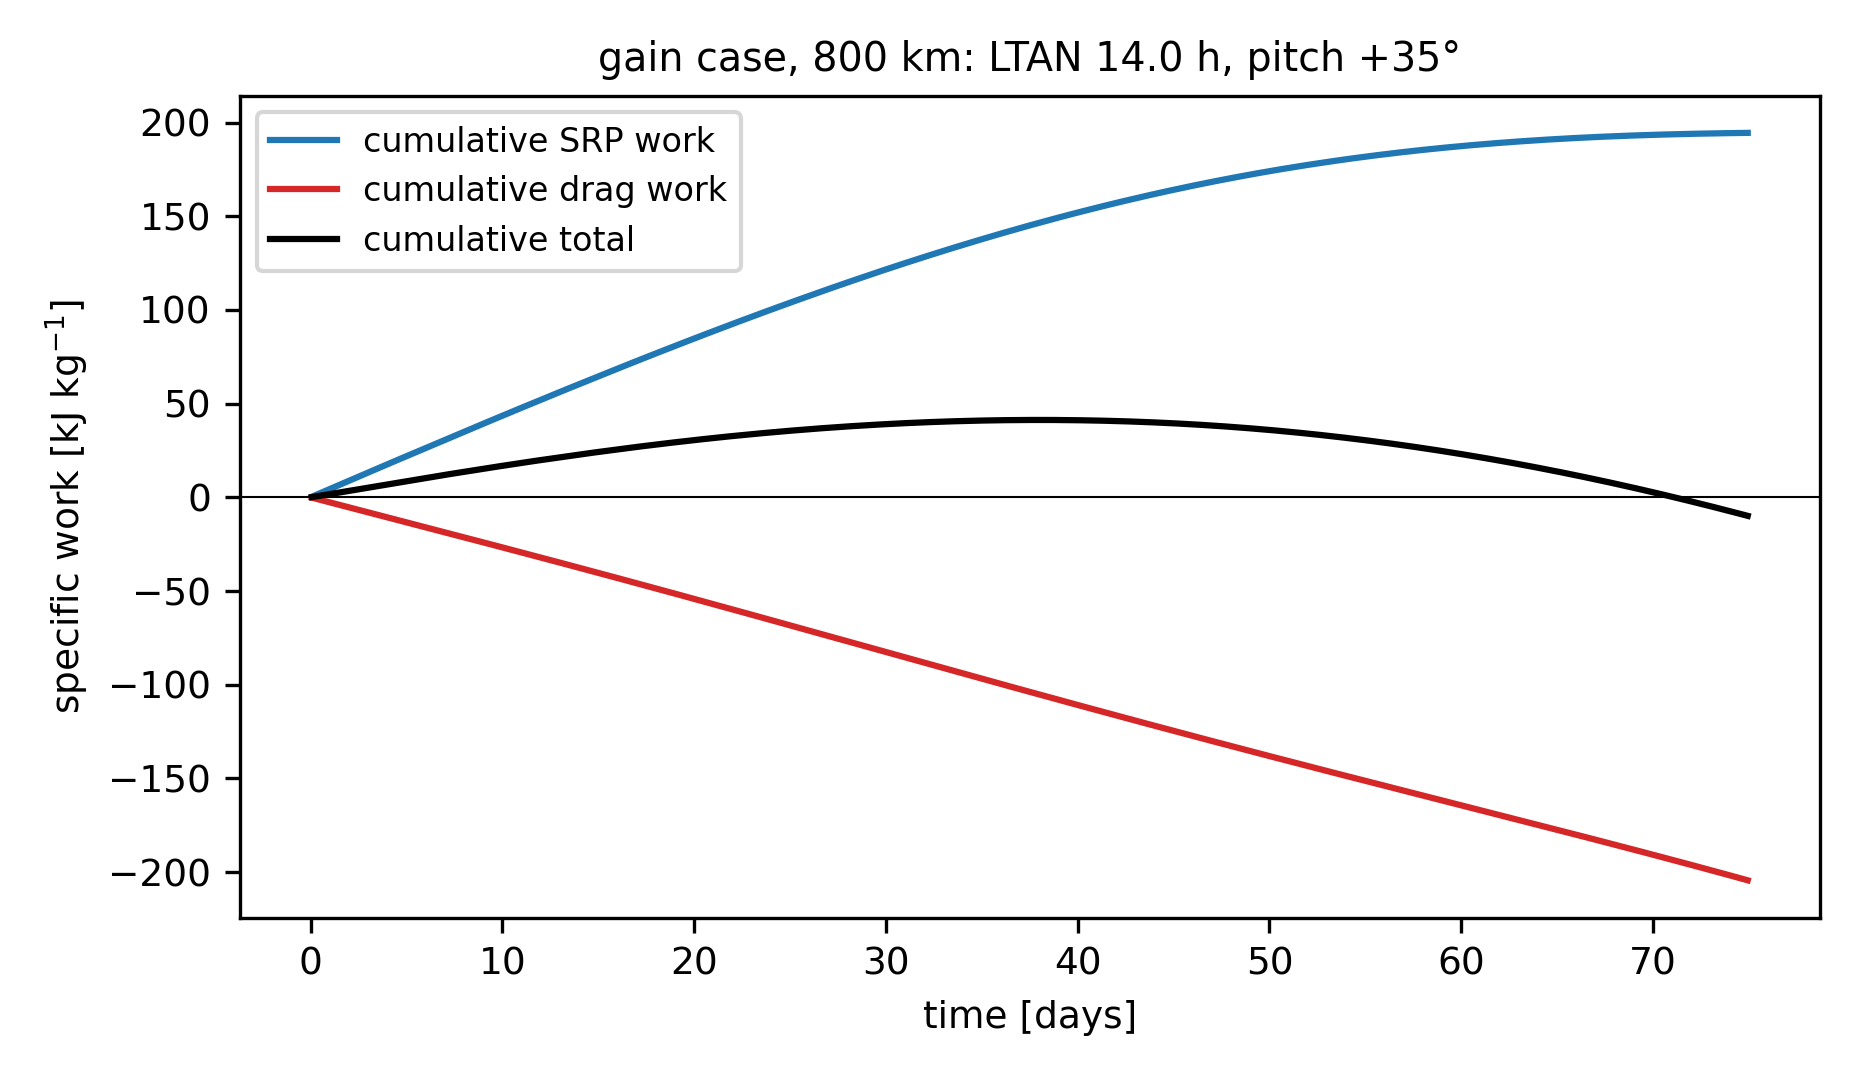
\includegraphics[width=0.8\linewidth]{Figures/r_cum_work_75d.png}
    \setlength{\abovecaptionskip}{0pt}
    \caption{Cumulative specific SRP work, drag work and total work (\(\mathrm{kJ\,kg^{-1}}\)) for the representative \(800\,\mathrm{km}\) gain case over \(75\) days. The cumulative total peaks at \(+41.3\,\mathrm{kJ\,kg^{-1}}\) on day \(38.1\) and turns negative on day \(71.2\); by day \(75\) cumulative drag exceeds cumulative SRP work by \(5.1\%\).}
    \label{fig:gaincase_cumulative_work_budget}
\end{figure}

\vspace{5pt}
\par\noindent The more revealing diagnostic is the orbit-averaged early-versus-late comparison in the left panel of Figure~\ref{fig:gaincase_early_late_work_comparison} and in Table~\ref{tab:gaincase_earlylate_comparison}, which compares the first and last \(20\%\) of the run (\(214\) of \(1069\) orbits each). Early in the run the mean SRP contribution of \(+301.3\,\mathrm{J\,kg^{-1}\,orbit^{-1}}\) exceeds the mean drag loss of \(-188.3\,\mathrm{J\,kg^{-1}\,orbit^{-1}}\), so the per-orbit balance is \(+113.0\,\mathrm{J\,kg^{-1}\,orbit^{-1}}\). Late in the run the mean SRP contribution has collapsed to \(+33.2\,\mathrm{J\,kg^{-1}\,orbit^{-1}}\), a factor of \(0.110\) of its early value, while the drag loss is essentially unchanged at \(-187.6\,\mathrm{J\,kg^{-1}\,orbit^{-1}}\) (ratio \(0.996\)); the net balance is \(-154.4\,\mathrm{J\,kg^{-1}\,orbit^{-1}}\). The per-orbit net work first turns negative on day \(38.1\), at orbit \(543\), which is exactly the peak of mean \(a\): the peak is simply the point at which the local balance changes sign, and everything after it is decay. Two features of this comparison deserve emphasis. First, the drag loss per orbit is almost identical in the two windows, so the deterioration of the balance is driven entirely by the loss of SRP work rather than by growth of the drag penalty; perigee erosion matters because it concentrates that penalty near perigee and leaves the orbit less able to tolerate the loss, as the decay case shows, not because it enlarges the penalty within this window. Second, the eclipse fraction per orbit barely changes, \(0.323\) early against \(0.330\) late, so the loss of SRP work is not a consequence of changing eclipse geometry. Its cause lies in the attitude.

\begin{table*}[htbp]
\centering
\caption{Early-versus-late comparison for the representative \(800\,\mathrm{km}\) gain case. The orbit-averaged work budget and eclipse fraction use \(20\%\) windows (first and last \(214\) of \(1069\) orbits); the orbit-mean SRP acceleration components use \(10\%\) windows (first and last \(107\) orbits), matching the conventions of the figure-generation scripts. \(|a_T|\) and \(|a_N|\) are the transverse and normal components of the SRP acceleration in the local orbital frame of Section~\ref{sec:model}; \(\alpha\) is the angle between the Sun line and the inertially fixed sail normal, quoted at day \(0\) and day \(75\).}
\label{tab:gaincase_earlylate_comparison}
\small
\begin{tabular}{p{5.8cm} p{1.9cm} p{1.9cm} p{1.8cm}}
\toprule
Metric & Early window & Late window & Late / Early \\
\midrule
\multicolumn{4}{l}{\textit{Orbit-averaged work budget (\(20\%\) windows; \(214\) orbits each)}} \\
Mean SRP work [J\,kg\(^{-1}\)\,orbit\(^{-1}\)]
& \(+301.3\)
& \(+33.2\)
& 0.110 \\

Mean drag work [J\,kg\(^{-1}\)\,orbit\(^{-1}\)]
& \(-188.3\)
& \(-187.6\)
& 0.996 \\

Mean net work [J\,kg\(^{-1}\)\,orbit\(^{-1}\)]
& \(+113.0\)
& \(-154.4\)
& --- \\

Eclipse fraction per orbit
& 0.323
& 0.330
& --- \\

\addlinespace
\multicolumn{4}{l}{\textit{SRP acceleration projection (\(10\%\) windows; \(107\) orbits each)}} \\
Orbit-mean \(\left|a_T\right|\) [\(\mu\mathrm{m\,s^{-2}}\)]
& \(21.6\)
& \(1.08\)
& 0.050 \\

Orbit-mean \(\left|a_N\right|\) [\(\mu\mathrm{m\,s^{-2}}\)]
& \(17.0\)
& \(1.49\)
& 0.088 \\

Ratio \(\left|a_N\right|/\left|a_T\right|\)
& 0.79
& 1.38
& --- \\

\addlinespace
\multicolumn{4}{l}{\textit{Sun--normal geometry (day \(0\) and day \(75\))}} \\
Sun--normal angle, \(\alpha\) [deg]
& 35.0
& 83.4
& --- \\

\(\cos^2\alpha\)
& 0.671
& 0.013
& --- \\
\bottomrule
\end{tabular}
\end{table*}

\vspace{5pt}
\par\noindent The late-time weakening follows directly from the SRP model and the force-decomposition framework of Section~\ref{sec:model}. There, using the Gauss Variational Equations, we argued that semi-major-axis growth depends on maintaining a favourable in-plane forcing, in particular a strong transverse component \(F_T\), while the normal component \(F_N\) contributes nothing directly to the energy. The sail normal is held fixed in inertial space, but the Sun moves along the ecliptic at roughly \(1^\circ\) per day and the Sun-synchronous orbit plane precesses with it, so the Sun--normal angle \(\alpha\) opens steadily: from \(35.0^\circ\) at day \(0\) to \(39.4^\circ\) on day \(14\), \(48.6^\circ\) on day \(30\), \(54.2^\circ\) on day \(38\), \(59.4^\circ\) on day \(45\), \(71.2^\circ\) on day \(60\) and \(83.4^\circ\) on day \(75\). Since the specular force scales with \(\cos^2\alpha\), which falls from \(0.671\) to \(0.013\) over the run, the SRP acceleration on the sail is reduced by a factor of about fifty. The right panel of Figure~\ref{fig:gaincase_early_late_work_comparison} shows the result in the orbital frame: over the first and last \(10\%\) windows (\(107\) orbits each) the orbit-mean transverse component \(|a_T|\) falls from \(21.6\) to \(1.08\,\mu\mathrm{m\,s^{-2}}\), a factor of \(0.050\), and the orbit-mean normal component \(|a_N|\) falls from \(17.0\) to \(1.49\,\mu\mathrm{m\,s^{-2}}\), a factor of \(0.088\). The SRP force therefore does not merely redistribute between the transverse and normal channels; its magnitude collapses, and what remains projects relatively more into the normal channel, with \(|a_N|/|a_T|\) rising from \(0.79\) to \(1.38\). The transverse forcing that generates \(\dot{a}\) is thus doubly penalised, by the overall loss of illumination and by the less favourable projection of what is left.

\begin{figure*}[htbp]
    \centering
    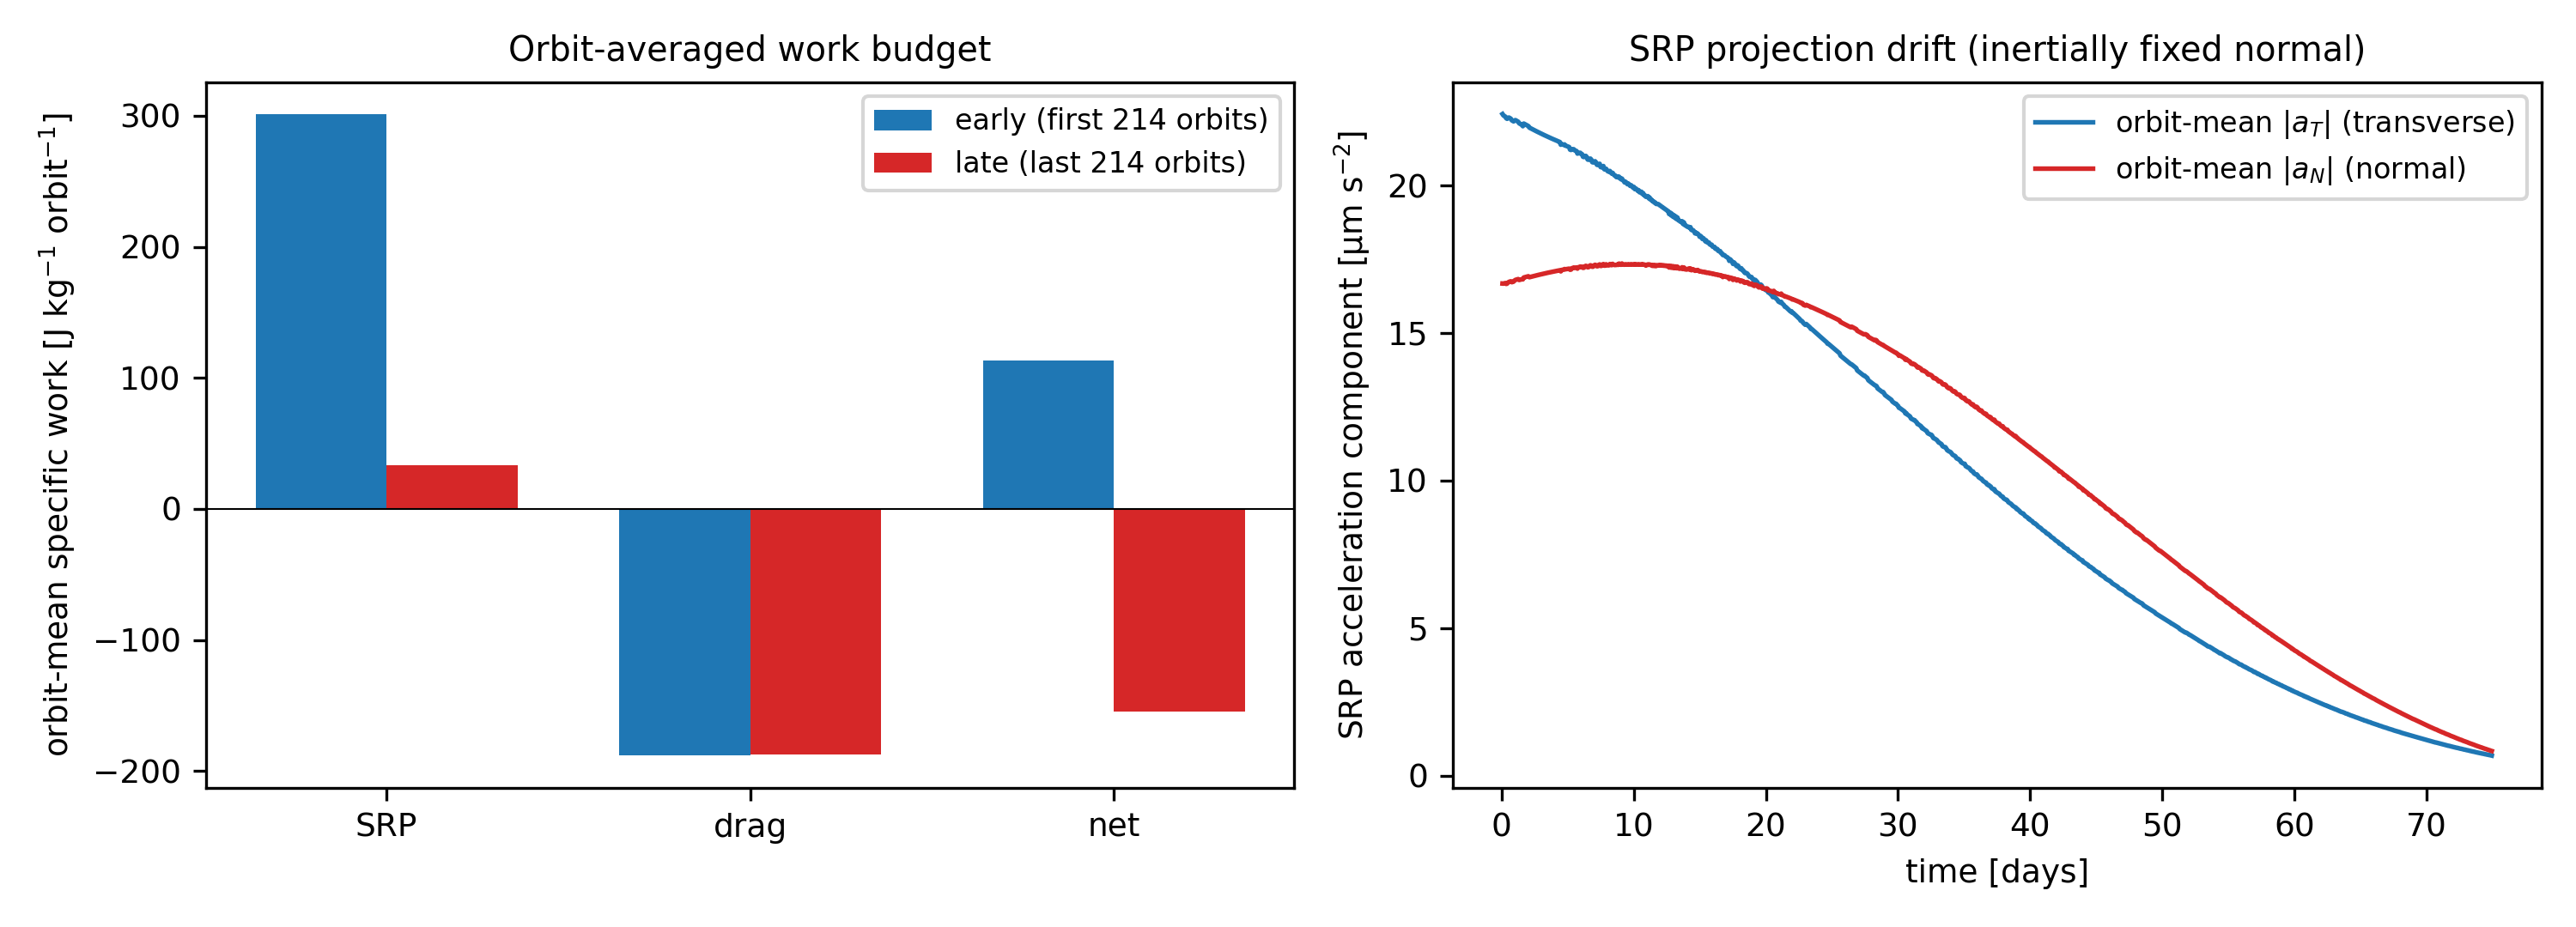
\includegraphics[width=1\linewidth]{Figures/r_earlylate_ftfn.png}
    \setlength{\abovecaptionskip}{0pt}
    \caption{Early-versus-late diagnostics for the representative \(800\,\mathrm{km}\) gain case. Left: orbit-averaged specific SRP, drag and net work (\(\mathrm{J\,kg^{-1}\,orbit^{-1}}\)) in the first and last \(20\%\) windows (\(214\) orbits each); the SRP contribution collapses while the drag penalty is unchanged, so the late-window net balance is negative. Right: orbit-mean transverse \(|a_T|\) and normal \(|a_N|\) components of the SRP acceleration (\(\mu\mathrm{m\,s^{-2}}\)) as functions of time; both fall by more than an order of magnitude as the inertially fixed sail normal drifts away from the Sun line.}
    \label{fig:gaincase_early_late_work_comparison}
\end{figure*}

\vspace{5pt}
\par\noindent This attitude drift is not secondary bookkeeping; it is the dominant late-time effect. Figure~\ref{fig:precession_drift} sketches the geometry. A spin-stabilised sail with its normal fixed in inertial space is well aligned with the Sun at the start of the run, when the pitch of \(+35^\circ\) places the SRP force favourably in the local RT plane during the sunlit arc. Two months later the Sun has moved some \(60^\circ\) along the ecliptic and the orbit plane has precessed with it, while the sail normal has not moved at all. The same inertially fixed attitude therefore sees the Sun at a grazing angle and projects what little force remains less favourably into the local frame. The mechanism established in Section~\ref{sec:existence} requires both the eclipse-induced sign selectivity and a sail that faces the Sun; the first is preserved over \(75\) days, but the second is lost by any attitude that is not actively steered. This is the second breakdown pathway, and in this case the stronger one.

\begin{figure*}[htbp]
    \centering
    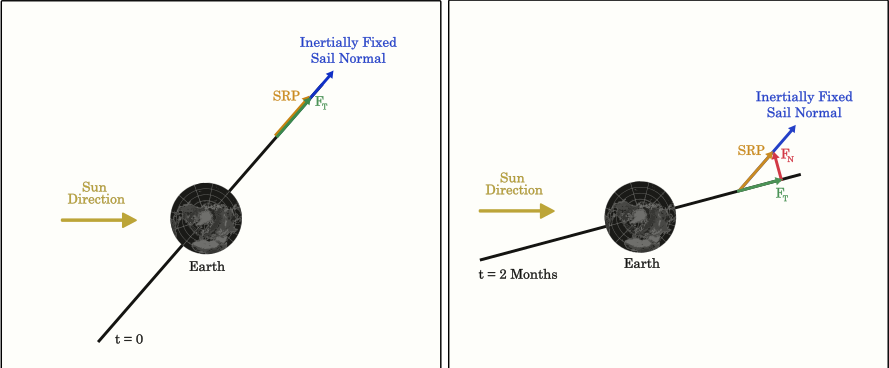
\includegraphics[width=1\linewidth]{Figures/precession.png}
    \caption{Illustration of SRP projection drift for an inertially fixed, spin-stabilised sail in a precessing Sun-synchronous orbit. At \(t=0\) (left), the fixed sail normal is \(35^\circ\) from the Sun line and produces a favourable transverse SRP component \(F_T\). After two months (right), the Sun has moved along the ecliptic and the orbit plane has precessed with it, so the same inertially fixed attitude is illuminated at a grazing angle and projects less favourably into the local frame, with a much reduced \(F_T\) and a relatively larger normal contribution \(F_N\). This geometric drift is the dominant cause of the breakdown of the transient gain regime over the \(75\)-day horizon.}
    \label{fig:precession_drift}
\end{figure*}

\vspace{5pt}
\par\noindent Taken together, the results in this section resolve the apparent tension between early gain and later decay. The mechanism established in Section~\ref{sec:existence} is real, but it is front-loaded and self-limiting. The early positive \(\Delta a\) is achieved mainly through apogee pumping rather than clean whole-orbit lifting; that evolution increases eccentricity and lowers perigee by some \(90\,\mathrm{km}\), which concentrates drag loss, while the inertially fixed sail orientation causes the SRP acceleration to shrink by a factor of about fifty as the Sun--normal angle opens from \(35.0^\circ\) to \(83.4^\circ\). The orbit-averaged balance turns negative on day \(38.1\), at the peak \(\Delta a_{\max,75\mathrm{d}} = +10.86\,\mathrm{km}\); mean \(a\) returns to its initial value on day \(71.0\); and by day \(75\) the cumulative total work is \(-9.9\,\mathrm{kJ\,kg^{-1}}\) with \(\Delta a_{75\mathrm{d}} = -2.69\,\mathrm{km}\). The regime does not fail abruptly; it progressively exhausts the margin that created it, and within the analysed window it exhausts that margin completely. How sensitive this behaviour is to the geometric and physical parameters of the case is the question taken up in Section~\ref{sec:sensitivity}.

\FloatBarrier
